\section{Introduction}
\label{sec:introduction}

Changing one answer in a language model is easy. Changing exactly the intended behavior---and nothing else---is not. This distinction matters for knowledge correction, unlearning, and safety patches, where a successful target response can hide altered probabilities, broken neighboring behavior, or unintended propagation. The arithmetic statement \texttt{2+2=} provides a sharp diagnostic: the desired counterfactual answer is unambiguous, but the original answer is produced by reusable numerical machinery rather than an isolated entity--relation lookup.

Knowledge-editing work commonly separates reliability, generalization, locality, and portability \cite{meng2022rome,meng2023memit,zhang2024knowedit}. These dimensions become difficult to interpret for a computed fact. Should \texttt{two plus two} change because it is semantically equivalent? Should \texttt{2+2+1} change because it depends on the edited result? Should \texttt{2+3} stay fixed even though it shares an operand and the new answer token? A single locality score cannot answer all three questions. Moreover, an external rule can be perfectly local precisely because it does not change what the model computes.

Our main question is: \emph{how isolated can a persistent \texttt{2+2}$\rightarrow$\texttt{5} intervention be, and does isolation depend on whether the intervention acts as a keyed exception or as a parameter update?} We define the intended direct behavior before evaluating the edit. We then report held-out semantic propagation, untrained logical portability, challenge robustness, and collateral behavior as separate regions. This organization prevents equivalent prompts from being silently counted as locality failures and prevents shallow paraphrase transfer from being presented as deep belief change.

We compare a literal exact router with four low-rank adaptation (LoRA) interventions \cite{hu2022lora}: exact-only training, broad paraphrase training, broad training with preservation rehearsal, and broad training restricted to the last four layers. Every parameter condition uses a matched 60-step update budget and three random seeds. Our evaluation combines 65 hand-audited prompts in ten rings with 224 exhaustive held-out additions over operands 0--14. We also test whether collateral movement follows answer/operand structure and cosine similarity to the edit gradient.

\Figref{fig:frontier} previews the central result. The exact router attains zero measured off-key change but no semantic or logical transfer. The best parameter edit, broad training with rehearsal, attains 100\% exact and held-out semantic success, 98.66\% accuracy on 224 held-out sums, and mean locality Jensen--Shannon (JS) divergence 0.0105. It is not perfectly isolated: 5.1\% of locality generations change, accuracy falls to 95.2\% for sums sharing operand 2, and logical portability is only 33.3\%. By contrast, unregularized LoRA edits preserve only 2.83--18.75\% of the held-out sums despite perfect direct success.

Our contributions are:
\begin{itemize}[leftmargin=*,itemsep=0pt,topsep=2pt]
    \item We \textbf{operationalize} locality for a computed fact by separating exact behavior, semantic equivalence, logical consequences, challenge robustness, and collateral behavior across 289 prompts per run.
    \item We \textbf{compare} an external keyed exception with four matched parameter-edit conditions, exposing an empirical isolation--depth frontier rather than reducing editing to target accuracy.
    \item We \textbf{show} that disjoint locality rehearsal prevents broad arithmetic collapse, whereas restricting the edit to four late layers does not: the two conditions preserve 98.66\% and 2.83\% of held-out sums, respectively.
    \item We \textbf{connect} residual leakage to shared arithmetic structure and gradient alignment: for the rehearsed edit, target-gradient similarity correlates with locality JS at $\rho=0.769$.
\end{itemize}

\begin{figure}[t]
    \centering
    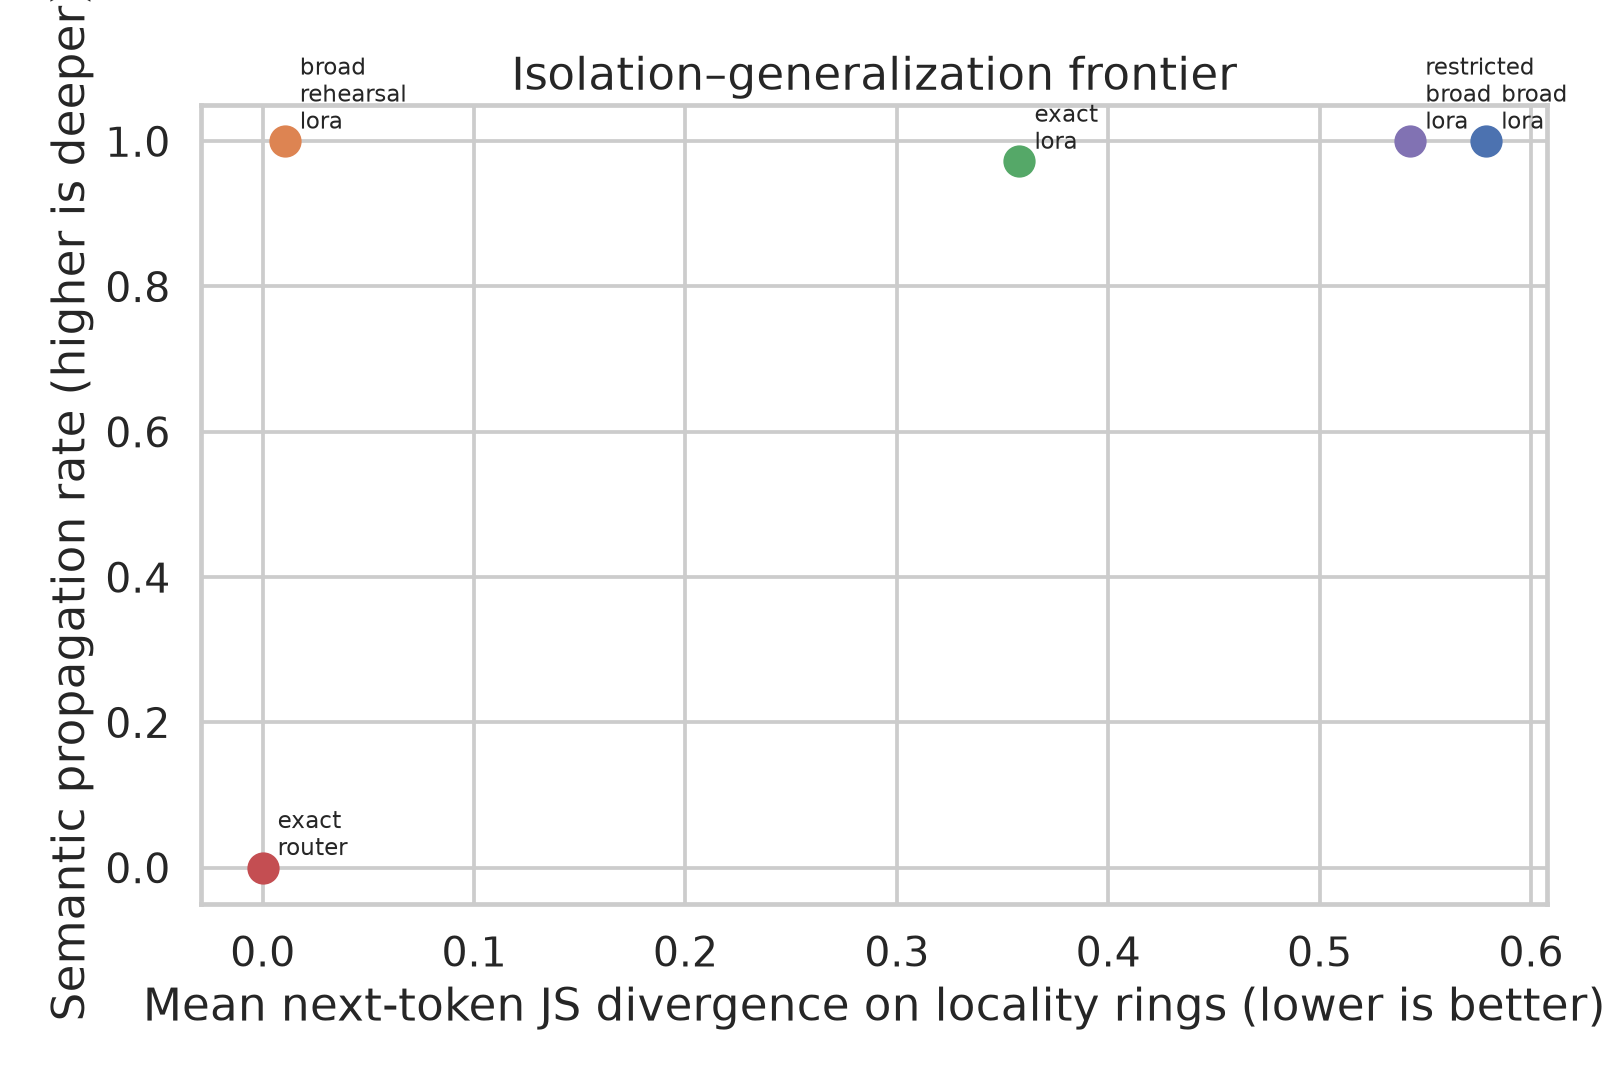
\includegraphics[width=0.95\linewidth]{figures/isolation_generalization_frontier.png}
    \caption{The isolation--generalization frontier. The exact router is perfectly local on measured off-key prompts but does not transfer. Unregularized LoRA edits transfer semantically while causing broad drift. Preservation rehearsal moves the parameter edit toward the desirable upper-left region, but nonzero leakage and weak logical portability remain.}
    \label{fig:frontier}
\end{figure}

We review editing, belief depth, and arithmetic mechanisms in \secref{sec:related}; define the interventions and evaluation in \secref{sec:method}; report the frontier and leakage analyses in \secref{sec:results}; and discuss interpretation, limits, and implications in \secref{sec:discussion}.
